\documentclass{article}
\usepackage[utf8]{inputenc}
\usepackage[UKenglish]{babel}
\usepackage[UKenglish]{isodate}
\usepackage{fullpage}
\usepackage{amsthm}
\usepackage{amsfonts}
\usepackage{amsmath}
\usepackage{mathtools}
\usepackage[capitalise]{cleveref}
\usepackage{bm}
\usepackage{booktabs}
\usepackage{tikz}
\usepackage{xcolor}
\usepackage[backgroundcolor=lightgray]{todonotes}
\usepackage{complexity}

\newtheorem{theorem}{Theorem}
\newtheorem{lemma}[theorem]{Lemma}
\newtheorem{proposition}[theorem]{Proposition}
\newtheorem{corollary}[theorem]{Corollary}
\newtheorem{conjecture}[theorem]{Conjecture}
\theoremstyle{definition}
\newtheorem{definition}[theorem]{Definition}
\newtheorem{example}[theorem]{Example}
\theoremstyle{remark}
\newtheorem*{remark}{Remark}

\Crefname{property}{Property}{Properties}
\Crefname{condition}{Condition}{Conditions}
\creflabelformat{condition}{#2(#1)#3}

\DeclareMathOperator{\WMC}{WMC}
\DeclareMathOperator{\nWMC}{NWMC}
\DeclareMathOperator{\id}{id}
\DeclareMathOperator{\End}{End}

\usetikzlibrary{cd}
\usetikzlibrary{bayesnet}
\usetikzlibrary{calc}

\tikzset{
  Subset/.style={
    draw=none,
    every to/.append style={
      edge node={node [sloped, allow upside down, auto=false]{$\subset$}}}
  }
}

\title{What Boolean Algebras Can Teach Us About Weighted Model Counting}
%\title{Generalising Weighted Model Counting to Boolean Algebras}
%\title{On the Limitations of Weighted Model Counting}
%\title{Weighted Model Counting/Integration from the Perspective of Boolean Algebras}
%\title{What Boolean Algebras Can Teach Us About Weighted Model Counting/Integration?}
\author{Paulius Dilkas}

\begin{document}
\maketitle

\section{Introduction}
% Feedback: What are the main claims, what are the main takeaways, intuitive
% [???] of theorems to follow. To do this, we appeal to algebraic constructions
% to define the main concepts for introducing measures on Boolean algebras.

% Feedback: Can you say something here about factorized vs non-factorized
% weight function definitions? That is, factorized is when w maps literals to
% R_>=0, non-factorized is when w maps models to R_>=0 and show:
% a) come up with nice example when non-factorized weights are intuitive
% c) clarify that the factorized definition have is w.r.t. models, in case some
% one gets confused [It doesn't have to be, if the BA is not free -- P.]

% Feedback 2: The paper at this stage is very technical - the danger is that
% WMC/SRL people may not be able to follow it and so would be hard to get
% accepted. Without clear target audience, [???] get work accepted. My main high
% level suggestion is that let us tease apart what you have and see if a story
% emerges. That is, let us attempt to write a paper *with examples* and see
% whether with significant motivation, we have a story emerging. Below, sample
% text needed to adequately motivate [???] for WMC/SRL community.

% Feedback from the panel: Clear up questions about independence between
% literals.

% TODO for later:
% 1) make up my mind about a,b vs x,y and stick to it (maybe x,y?)
% 2) Coproducts/pushouts vs (amalgamated) free products. Probably the former.
% 3) 'with generating set S' -> 'over S'

\paragraph{Contributions.}
\begin{itemize}
\item WMC defines a measure over a BA.
\item WMC with weights on literals imposes an independence assumption. (Measures
  are `slightly' more expressive than WMC with weights on models because they
  apply to non-atomic BAs.)
\item A BA can be augmented with new literals in order to support any measure.
\item (Maybe) a lower bound on the number of new literals needed in order to
  support any measure.
\item Alternatively, one can use coproducts and pushouts to define a BA with
  precisely the right independence and conditional independence conditions.
  (This requires a relaxed version of WMC.)
\item This results in a smaller problem for WMC algorithms (w.r.t. both the
  number of literals and the length of the theory) and is optimal for, e.g.,
  Bayesian networks.
\item (Maybe) this results in faster inference (?)
\end{itemize}

\paragraph{Notable previous/related work.}
\begin{itemize}
\item Hailperin's approach to probability logic
  \cite{DBLP:journals/ndjfl/Hailperin84}
\item Nilsson's (somewhat successful) probabilistic logic
  \cite{DBLP:journals/ai/Nilsson86}
\item Logical induction: a big paper with a good overview of previous attempts
  to assign probabilities to logical sentences in a sensible way
  \cite{DBLP:journals/eccc/GarrabrantBCST16}
\item Measures on Boolean algebras
  \begin{itemize}
  \item On possibility and probability measures in finite Boolean algebras
    \cite{DBLP:journals/soco/CastineiraCT02}
  \item Representation of conditional probability measures
    \cite{krauss1968representation}
  \end{itemize}
\end{itemize}

\section{Preliminaries}

% TODO
% 1) Feedback 2: Explain with examples: models = elements [atoms] of algebra
% 2) Perhaps reorder the section of preliminaries into paragraphs, i.e., a
% paragraph for order, for homomorphisms, etc. This would take up less space.
% 3) how to compute the number of elements in the algebra.

\begin{definition} \label{def:ba}
  A \emph{Boolean algebra} (BA) is a tuple $(\mathbf{B}, \land, \lor, \neg, 0,
  1)$ consisting of a set $\mathbf{B}$ with binary operations \emph{meet}
  $\land$ and \emph{join} $\lor$, unary operation $\neg$ and elements $0, 1 \in
  \mathbf{B}$ such that the following axioms hold for all $a, b, \in
  \mathbf{B}$:
  \begin{itemize}
  \item both $\land$ and $\lor$ are associative and commutative;
  \item $a \lor (a \land b) = a$, and $a \land (a \lor b) = a$;
  \item $0$ is the identity of $\lor$, and $1$ is the identity of $\land$;
  \item $\lor$ distributes over $\land$ and vice versa;
  \item $a \lor \neg a = 1$, and $a \land \neg a = 0$.
  \end{itemize}
\end{definition}

For clarity and succinctness, we will occasionally use three other operations
that can be defined using the original three\footnote{We use $+$ to denote
  symmetric difference because it is the additive operation of a Boolean ring.}:
\begin{align*}
  a \to b &= \neg a \lor b, \\
  a \leftrightarrow b &= (a \land b) \lor (\neg a \land \neg b), \\
  a + b &= (a \land \neg b) \lor (\neg a \land b).
\end{align*}
We can also define a partial order $\le$ on $\mathbf{B}$ as $a \le b$ if $a = b
\land a$ (or, equivalently, $a \lor b = b$) for all $a, b \in \mathbf{B}$.
Furthermore, let $a < b$ denote $a \le b$ and $a \ne b$. For the rest of this
paper, let $\mathbf{B}$ refer to the BA $(\mathbf{B}, \land, \lor, \neg, 0, 1)$.
For any $S \subseteq \mathbf{B}$, we write $\bigvee S$ for $\bigvee_{x \in S} x$
and call it the \emph{supremum} of $S$. Similarly, $\bigwedge S = \bigwedge_{x
  \in S} x$ is the \emph{infimum}. By convention, $\bigwedge \emptyset = 1$ and
$\bigvee \emptyset = 0$. For any $a, b \in \mathbf{B}$, we say that $a$ and $b$
are \emph{disjoint} if $a \land b = 0$.

\begin{definition}[\cite{DBLP:books/daglib/0090259,levasseur2012applied}]
  An element $a \ne 0$ of $\mathbf{B}$ is an \emph{atom} if, for all $x \in
  \mathbf{B}$, either $x \land a = a$ or $x \land a = 0$. Equivalently, $a \ne
  0$ is an atom if there is no $x \in \mathbf{B}$ such that $0 < x < a$. We say
  that $\mathbf{B}$ is \emph{atomic} if for every $a \in \mathbf{B} \setminus \{0
  \}$, there is an atom $x$ such that $x \le a$.
\end{definition}

\begin{lemma}[\cite{ganesh2006introduction}]
  For any two distinct atoms $a$, $b \in \mathbf{B}$, $a \land b = 0$.
\end{lemma}

\begin{lemma}[\cite{givant2008introduction}] \label{thm:representation}
  The following are equivalent:
  \begin{itemize}
  \item $\mathbf{B}$ is atomic.
  \item For any $x \in \mathbf{B}$, $x = \bigvee_{\text{atoms } a \le x} a$.
  \item $1$ is the supremum of all atoms.
  \end{itemize}
\end{lemma}

\begin{lemma}[\cite{givant2008introduction}] \label{lemma:atomic}
  All finite BAs are atomic.
\end{lemma}

\begin{definition}[\cite{gaifman1964concerning,DBLP:books/daglib/0090259}] \label{def:measure}
  A \emph{measure} on $\mathbf{B}$ is a function $m\colon
  \mathbf{B} \to \mathbb{R}_{\ge 0}$ such that:
  \begin{itemize}
  \item $m(0) = 0$;
  \item $m(a \lor b) = m(a) + m(b)$ for all $a, b \in \mathbf{B}$ whenever $a
    \land b = 0$.
  \end{itemize}
  If $m(1) = 1$, we call $m$ a \emph{probability measure}. Also, if $m(x) > 0$
  for all $x \ne 0$, then $m$ is \emph{strictly positive}.
\end{definition}

\begin{definition}[\cite{givant2008introduction}]
  Let $\mathbf{A}$ and $\mathbf{B}$ be BAs. A \emph{(Boolean) homomorphism} from
  $\mathbf{A}$ to $\mathbf{B}$ is a map $f\colon \mathbf{A} \to \mathbf{B}$ such
  that:
  \begin{itemize}
  \item $f(x \land y) = f(x) \land f(y)$,
  \item $f(x \lor y) = f(x) \lor f(y)$,
  \item $f(\neg x) = \neg f(x)$
  \end{itemize}
  for all $x, y \in \mathbf{A}$.
\end{definition}

\begin{lemma}[Homomorphisms preserve order
  \cite{givant2008introduction}] \label{lemma:homomorphisms_and_order}
  Let $f\colon \mathbf{A} \to \mathbf{B}$ be a homomorphism between two BAs
  $\mathbf{A}$ and $\mathbf{B}$. Then, for any $x, y \in \mathbf{A}$, if $x \le
  y$, then $f(x) \le f(y)$.
\end{lemma}

\begin{lemma}[\cite{sikorski1969boolean}] \label{lemma:order}
  For any $a, b \in \mathbf{B}$, $a \le b$ if and only if $a \land \neg b = 0$.
\end{lemma}

\begin{lemma}[\cite{givant2008introduction}] \label{lemma:measure_and_order}
  Let $m\colon \mathbf{B} \to \mathbb{R}_{\ge 0}$ be a measure. Then for all $a,
  b \in \mathbf{B}$, if $a \le b$, then $m(a) \le m(b)$.
\end{lemma}

\begin{definition}[\cite{koppelberg1989handbook}]
  Let $S$ be a set, and let $\mathbf{B}$ be a BA. Then $\mathbf{B}$ is a
  \emph{free BA over $S$} if there is a map $S \to \mathbf{B}$ such that for any
  BA $\mathbf{C}$ and map $S \to \mathbf{C}$, there is a unique homomorphism
  $\mathbf{B} \to \mathbf{C}$ that makes
  \[
    \begin{tikzcd}
      S \ar[rd] \ar[r] & \mathbf{B} \ar[d,dashed] \\
      & \mathbf{C}.
    \end{tikzcd}
  \]
  commute. A BA $\mathbf{B}$ is \emph{free} if $S$ exists.
\end{definition}

\begin{lemma}[\cite{sikorski1969boolean}] \label{lemma:finite_and_free}
  A finite BA is free if and only if it has $2^{2^n}$ elements for some $n \in
  \mathbb{N}$. It then has $2^n$ atoms and $n$ generators.
\end{lemma}

\section{WMC as a Measure}
% TODO: Feedback 2: Need to explain how WMC and NWMC connects to standard
% definitions of WMC and Pr(phi|e) = WMC(phi /\ e)/WMC(e).

\begin{definition} \label{def:algebra_from_logic}
  Let $\mathcal{L}$ be a propositional (or first-order) logic, and let
  $\Delta$ be a theory in $\mathcal{L}$. We can define an equivalence
  relation on formulas in $\mathcal{L}$ as
  \[
    \alpha \sim \beta \quad \text{if and only if} \quad \Delta \vdash \alpha
    \leftrightarrow \beta
  \]
  for all $\alpha, \beta \in \mathcal{L}$. Let $[\alpha]$ denote the equivalence
  class of $\alpha \in \mathcal{L}$ with respect to $\sim$. We can then let
  $B(\Delta) = \{ [\alpha] \mid \alpha \in \mathcal{L} \}$ and define the
  structure of a BA on $B(\Delta)$ as
  \begin{align*}
    [\alpha] \lor [\beta] &= [\alpha \lor \beta], \\
    [\alpha] \land [\beta] &= [\alpha \land \beta], \\
    \neg[\alpha] &= [\neg\alpha], \\
    1 &= [\alpha \to \alpha], \\
    0 &= [\alpha \land \neg\alpha]
  \end{align*}
  for all $\alpha, \beta \in \mathcal{L}$. Then $B(\Delta)$ is the
  \emph{Lindenbaum-Tarski algebra} of $\Delta$
  \cite{koppelberg1989handbook,tarski1983logic}.
\end{definition}

\begin{example} \label{example:construction}
  Let $\mathcal{L}$ be a propositional logic with $p$ and $q$ as its only atoms.
  Then $L = \{ p, q, \neg p, \neg q \}$ is its set of literals. Let $w : L \to
  \mathbb{R}_{\ge 0}$ be the \emph{weight function} defined by
  \begin{align*}
    w(p) = 0.3, \\
    w(\neg p) = 0.7, \\
    w(q) = 0.2, \\
    w(\neg q) = 0.8.
  \end{align*}
  Let $\Delta$ be a theory in $\mathcal{L}$ with a sole axiom $p$. Then
  $\Delta$ has two models, i.e., $\{ p, q \}$ and $\{ p, \neg q \}$. The
  \emph{weighted model count} (WMC) \cite{DBLP:journals/ai/ChaviraD08} of $\Delta$ is
  then
  \[
    \sum_{\omega \models \Delta} \prod_{\omega \models l} w(l) =
    w(p)w(q) + w(p)w(\neg q) = 0.3.
  \]

  % TODO: be careful about mentioning ideals, filters, and quotients
  The corresponding BA $B(\Delta)$ can then be constructed using
  \cref{def:algebra_from_logic}. Alternatively, one can first construct the free
  BA generated by the set $\{ p, q \}$ and then take a quotient with respect to
  either the filter generated by $p$ or the ideal\footnote{More details on these
    concepts can be found in many books on BAs
    \cite{givant2008introduction,koppelberg1989handbook}.} generated by $\neg
  p$.

  Each element of $B(\mathcal{L})$ can also be seen as a subset of the set of
  all models of $\mathcal{L}$, with $0$ representing $\emptyset$, $1$
  representing the set of all (four) models, each atom representing a single
  model, and each edge going upward representing a subset relation. Thus,
  the Boolean-algebraic way of calculating the WMC of $\Delta$ consists of:
  \begin{enumerate} % TODO: why is step 1 always possible?
  \item Identifying an element $a \in B(\mathcal{L})$ that corresponds to
    $\Delta$.
  \item Finding all atoms of $B(\mathcal{L})$ that are `dominated' by $a$
    according to the partial order.
  \item Using $w$ to calculate the weight of each such atom.
  \item Adding the weights of these atoms.
  \end{enumerate}
  This motivates the following definition of WMC generalised to BAs.
\end{example}
% TODO: clarify what B(L) means. And whether B(Delta) is even necessary.
% TODO: reference for the set/subset thing.

% TODO: Feedback 2: You need to explain what precisely these mean in logic and
% models and weight functions are usually defined and understood.
% TODO: This should be replaced with inner sums (a.k.a. free products)
\begin{definition} \label{def:wmc}
  Let $\mathbf{B}$ be an atomic BA, and let $M \subset \mathbf{B}$ be its set of
  atoms. Let $L \subset \mathbf{B}$ be such that every atom $m \in M$ can be
  uniquely expressed as $m = \bigwedge L'$ for some $L' \subseteq L$, and let
  $w\colon L \to \mathbb{R}_{\ge 0}$ be arbitrary. The \emph{weighted model
    count} $\WMC_w\colon \mathbf{B} \to \mathbb{R}_{\ge 0}$ is defined as
  \[
    \WMC_w(x) = \begin{cases}
      0 & \text{if } x = 0 \\
      \prod_{l \in L'} w(l) & \text{if } M \ni x = \bigwedge L' \\
      \sum_{\text{atoms } a \le x} \WMC_w(a) & \text{otherwise}
    \end{cases}
  \]
  for any $x \in \mathbf{B}$. Furthermore, we define the \emph{normalised
    weighted model count} $\nWMC_w\colon \mathbf{B} \to [0, 1]$ as $\nWMC_w(x) =
  \frac{\WMC_w(x)}{\WMC_w(1)}$ for all $x \in \mathbf{B}$. For both $\WMC_w$ and
  $\nWMC_w$, we will drop the subscript when doing so results in no potential
  confusion. Finally, we say that a measure $m\colon \mathbf{B} \to
  \mathbb{R}_{\ge 0}$ is a \emph{WMC measure} (or is \emph{WMC-definable}) if
  there exists a subset $L \subset \mathbf{B}$ and a weight function $w\colon L
  \to \mathbb{R}_{\ge 0}$ such that $m = \WMC_w$.
\end{definition}
% TODO: mention that the definition can be reduced to a single formula (i.e.,
% without cases)
% TODO: any measure is a WMC measure if all atoms are in L

\begin{theorem}
  $\WMC$ is a measure, and $\nWMC$ is a probability measure.
\end{theorem}
\begin{proof}
  First, note that $\WMC$ is non-negative and $\WMC(0) = 0$ by definition. Next,
  let $x, y \in \mathbf{B}$ be such that $x \land y = 0$. We want to show that
  \begin{equation} \label{eq:additivity_proof}
    \WMC(x \lor y) = \WMC(x) + \WMC(y).
  \end{equation}
  If, say, $x = 0$, then \cref{eq:additivity_proof} becomes
  \[
    \WMC(y) = \WMC(0) + \WMC(y) = \WMC(y)
  \]
  (and likewise for $y = 0$). Thus we can assume that $x \ne 0 \ne y$ and use
  \cref{thm:representation} to write
  \[
    x = \bigvee_{i \in I} x_i \quad \text{and} \quad y = \bigvee_{j \in J} y_j
  \]
  for some sequences of atoms $(x_i)_{i \in I}$ and $(y_j)_{j \in J}$. If
  $x_{i'} = y_{j'}$ for some $i' \in I$ and $j' \in J$, then
  \[
    x \land y = \bigvee_{i \in I} \bigvee_{j \in J} x_i \land y_j = x_{i'} \land
    y_{j'} \ne 0,
  \]
  contradicting the assumption. This is enough to show that
  \begin{align*}
    \WMC(x \lor y) &= \WMC\left( \left( \bigvee_{i \in I} x_i \right) \lor \left(\bigvee_{j \in J} y_j \right) \right) = \sum_{i \in I} \WMC(x_i) + \sum_{j \in J} \WMC(y_j) \\
                   &= \WMC(x) + \WMC(y),
  \end{align*}
  finishing the proof that $\WMC$ is a measure. This immediately shows that
  $\nWMC$ is a probability measure since, by definition, $\nWMC(1) = 1$.
\end{proof}

Given a theory $\Delta$ in a logic $\mathcal{L}$, the usual way of using WMC to
compute the probability of a query $q$ is
\cite{DBLP:conf/uai/Belle17,DBLP:conf/aaai/SangBK05}
\[
  \Pr_{\Delta, w}(q) = \frac{\WMC_w(\Delta \land q)}{\WMC_w(\Delta)}.
\]
In our algebraic formulation, this can be computed in two different ways:
\begin{itemize}
\item as $\frac{\WMC_w(\Delta \land q)}{\WMC_w(\Delta)}$ in $B(\mathcal{L})$,
\item and as $\nWMC_w([q])$ in $B(\Delta)$.
\end{itemize}
But how does the measure defined on $B(\mathcal{L})$ transfer to $B(\Delta)$?

\section{What Measures Are WMC-Definable?}

% TODO: Proofs need to be updated and propositions could be phrased in a better
% way, but the gist should be the same.

\subsection{WMC Requires Independent Literals}

\begin{lemma} \label{lemma:before_theorem}
  For any measure $m\colon \mathbf{B} \to \mathbb{R}_{\ge 0}$ and elements $a, b
  \in \mathbf{B}$,
  \begin{equation} \label{eq:to_prove}
    m(a \land b) = m(a)m(b)
  \end{equation}
  if and only if
  \begin{equation} \label{eq:to_prove2}
    m(a \land b) \cdot m(\neg a \land \neg b) = m(a \land \neg b)
    \cdot m(\neg a \land b).
  \end{equation}
\end{lemma}
\begin{proof}
  First, note that $a = (a \land b) \lor (a \land \neg b)$ and $(a \land b)
  \land (a \land \neg b) = 0$, so, by properties of a measure,
  \begin{equation} \label{eq:temp}
    m(a) = m(a \land b) + m(a \land \neg b).
  \end{equation}
  Applying \cref{eq:temp} and the equivalent expression for $m(b)$ allows us
  to rewrite \cref{eq:to_prove} as
  \[
    m(a \land b) = [m(a \land b) + m(a \land \neg b)][m(a \land b) + m(\neg a
    \land b)]
  \]
  which is equivalent to
  \begin{equation} \label{eq:temp6}
    m(a \land b)[1 - m(a \land b) - m(a \land \neg b) - m(\neg a \land b)] = m(a
    \land \neg b)m(\neg a \land b).
  \end{equation}
  Since $a \land b$, $a \land \neg b$, $\neg a \land b$, $\neg a \land \neg b$
  are pairwise disjoint and their supremum is $1$,
  \[
    m(a \land b) + m(a \land \neg b) + m(\neg a \land b) + m(\neg a \land \neg
    b) = 1,
  \]
  and this allows us to rewrite \cref{eq:temp6} into \cref{eq:to_prove2}. As all
  transformations are invertible, the two expressions are equivalent.
\end{proof}

% TODO: a special case for weight=0.
\begin{theorem}
  Let $\mathbf{B}$ be a free BA over $\{ l_i \}_{i=1}^n$ (for some $n \in
  \mathbb{N}$) with measure $m\colon \mathbf{B} \to \mathbb{R}_{\ge 0}$, and let
  $L = \{ l_i \}_{i = 1}^n \cup \{ \neg l_i \}_{i = 1}^n$. Then there exists a
  weight function $w\colon L \to \mathbb{R}_{\ge 0}$ such that $m = \WMC_w$ if
  and only if
  \begin{equation} \label{eq:wmccondition}
  m(l \land l') = m(l)m(l')
  \end{equation}
  for all distinct $l, l' \in L$ such that $l \ne \neg l'$.
\end{theorem}

\begin{remark}
  Note that if $n = 1$, then \cref{eq:wmccondition} is vacuously satisfied and
  so any valid measure can be expressed as WMC.
\end{remark}

\begin{proof}
  ($\Leftarrow$) Let $w\colon L \to \mathbb{R}_{\ge 0}$ be defined by
  \begin{equation} \label{eq:assumption}
    w(l) = m(l)
  \end{equation}
  for all $l \in L$. We are going to show that $\WMC_w = m$. First, note that
  $\WMC_w(0) = 0 = m(0)$ by the definitions of both $\WMC_w$ and $m$. Second,
  let
  \begin{equation} \label{eq:def_of_a}
    a = \bigwedge_{i=1}^n a_i
  \end{equation}
  be an atom in $\mathbf{B}$ such that $a_i \in \{ l_i, \neg l_i \}$ for all $i
  \in [n]$. Then
  \[
    \WMC(a) = \prod_{i=1}^n w(a_i) = \prod_{i=1}^n m(a_i) = m
    \left(\bigwedge_{i=1}^n a_i \right) = m(a)
  \]
  by \cref{def:wmc,eq:assumption,eq:wmccondition,eq:def_of_a}. Finally, note
  that if $\WMC$ and $m$ agree on all atoms, then they must also agree on all
  other non-zero elements of the Boolean algebra.

  ($\Rightarrow$) For the other direction, we are given a weight function
  $w\colon L \to \mathbb{R}_{\ge 0}$ that induces a measure $m = \WMC_w\colon
  \mathbf{B} \to \mathbb{R}_{\ge 0}$, and we want to show that
  \cref{eq:wmccondition} is satisfied. Let $k_i, k_j \in L$ be such that $k_i
  \in \{ l_i, \neg l_i \}$, $k_j \in \{ l_j, \neg l_j \}$, and $i \ne j$ for
  some $i, j \in [n]$. We then want to show that
  \begin{equation} \label{eq:to_prove3}
    m(k_i \land k_j) = m(k_i)m(k_j)
  \end{equation}
  which is equivalent to
  \begin{equation} \label{eq:to_prove4}
    m(k_i \land k_j) \cdot m(\neg k_i \land \neg k_j) = m(k_i \land \neg k_j)
    \cdot m(\neg k_i \land k_j)
  \end{equation}
  by \cref{lemma:before_theorem}. Then
  \begin{align*}
    \WMC(k_i \land k_j) &= \sum_{\text{atoms } a \le k_i \land k_j} \WMC(a) = \sum_{\text{atoms } a \le k_i \land k_j} \prod_{m \in [n]} w(a_m) \\
                        &= \sum_{\text{atoms } a \le k_i \land k_j} w(a_i)w(a_j) \prod_{m \in [n] \setminus \{ i, j \}} w(a_m) = \sum_{\text{atoms } a \le k_i \land k_j} w(k_i)w(k_j) \prod_{m \in [n] \setminus \{ i, j \}} w(a_m) \\
    &= w(k_i)w(k_j) \sum_{\text{atoms } a \le k_i \land k_j} \prod_{m \in [n] \setminus \{ i, j \}} w(a_m) = w(k_i)w(k_j)C,
  \end{align*}
  where $C$ denotes the part of $\WMC(k_i \land k_j)$ that will be the same for
  $\WMC(\neg k_i \land k_j)$, $\WMC(k_i \land \neg k_j)$, and $\WMC(\neg k_i
  \land \neg k_j)$ as well. But then \cref{eq:to_prove4} becomes
  \[
    w(k_i)w(k_j)w(\neg k_i)w(\neg k_j)C^2 = w(k_i)w(\neg k_j)w(\neg k_i)w(k_j)C^2
  \]
  which is trivially true.
\end{proof}

\subsection{Extending the Algebra}

% TODO: Feedback 2: If you prove (b) above, you could motivate why weights on
% literals is attractive and whether there is a way to augment the expressivity
% of WMC while still maintaining literal level weights. Hence this action.

Given this requirement for independence, a well-known way to represent
probability distributions that do not consist entirely of independent variables
is by adding more literals \cite{DBLP:journals/ai/ChaviraD08}, i.e., extending
the set $L$ covered by the WMC weight function $w\colon L \to \mathbb{R}_{\ge
  0}$. Let us translate this idea to the language of BAs.

% TODO: If L denotes literals, then it doesn't denote a generating set
\begin{theorem} \label{thm:extension}
  Let $\mathbf{B}$ be a free BA over a finite set $S$, and let $m\colon
  \mathbf{B} \to \mathbb{R}_{\ge 0}$ be an arbitrary measure. Let $L = \{ s \mid
  s \in S \} \cup \{ \neg s \mid s \in S \}$. By \cref{lemma:finite_and_free},
  we know that $\mathbf{B}$ has $n = 2^{|S|}$ atoms. Let $\{a_i\}_{i=1}^n$
  denote those atoms in some arbitrary order. Let $L' = L \cup \{ \phi_i
  \}_{i=1}^n \cup \{\neg \phi_i \}_{i=1}^n$ be the set $L$ extended with $2n$
  new elements. Let $\mathbf{B'}$ be the unique Boolean algebra with $\{ \phi_i
  \land a_i \}_{i=1}^n \cup \{ \neg \phi_i \land a_i \}_{i=1}^n$ as its set of
  atoms. Let $\iota\colon \mathbf{B} \hookrightarrow \mathbf{B'}$ be the
  inclusion homomorphism. Let $w\colon L' \to \mathbb{R}_{\ge 0}$ be defined by
  \[
    w(l) = \begin{cases}
      m(a_i)/2 & \text{if } l = \phi_i \text{ or } l = \neg\phi_i \text{ for
        some } i \in [n] \\
      1 & \text{otherwise}
    \end{cases}
  \]
  for all $l \in L'$, and note that this defines a WMC measure $m' =
  \WMC_{w}\colon \mathbf{B'} \to \mathbb{R}_{\ge 0}$. Then
  \[
    m(a) = (m' \circ \iota)(a)
  \]
  for all $a \in \mathbf{B}$.
\end{theorem}

In other words, any measure can be computed using WMC by extending the BA with
more literals. More precisely, we are given the left-hand column in
\[
  \begin{tikzcd}
    \textcolor{red}{\mathbb{R}_{\ge 0}} & & \\
    \textcolor{red}{\mathbf{B}} \arrow[red]{u}{m} \ar[r,hookrightarrow,"\iota"]
    & \mathbf{B'} \arrow{lu}[swap]{m'} & \\
    \textcolor{red}{L} \ar[u,red,hookrightarrow] \ar[r,hookrightarrow] & L'
    \ar[u,hookrightarrow] \arrow{r}{w} & \mathbb{R}_{\ge 0}
  \end{tikzcd}
\]
and construct the remaining part in such a way that the triangle commutes.

% TODO: make J depend on i
\begin{proof} % TODO: find a reference for this first claim
  Since $\mathbf{B}$ is free over $S$, each atom $a_i \in \mathbf{B}$ is an
  infimum of elements in $L$, i.e.,
  \[
    a_i = \bigwedge_{j \in J} a_{i,j}
  \]
  for some $\{ a_{i,j} \}_{j \in J} \subset L$. Moreover, each atom $b \in
  \mathbf{B'}$ can be represented as either $b = \phi_i \land a_i$ or $b =
  \neg\phi_i \land a_i$ for some atom $a_i \in \mathbf{B}$, also making it an
  infimum over a subset of $L'$. Then, for any $b \in \mathbf{B}$,
  \[
    (m' \circ \iota)(b) = \sum_{\substack{\text{atoms } a_i \in \mathbf{B}:\\
        \phi_i \land a_i \le \iota(b)}} (w(\phi_i) + w(\neg\phi_i)) \prod_{j \in
    J} w(a_{i,j}),
  \]
  recognising that, for any $\iota(b)$, any atom $a_i \in \mathbf{B}$ satisfies
  $\phi_i \land a_i \le \iota(b)$ if and only if it satisfies $\neg\phi_i \land
  a_i \le \iota(b)$. Then, according to the definition of $w$,
  \[
    (m' \circ \iota)(b) = \sum_{\substack{\text{atoms } a_i \in \mathbf{B}:\\
        \phi_i \land a_i \le \iota(b)}} (w(\phi_i) + w(\neg\phi_i)) =
    \sum_{\substack{\text{atoms } a_i \in \mathbf{B}:\\ \phi_i \land a_i \le
        \iota(b)}} m(a_i) = m(b),
  \]
  provided that
  \[
    \phi_i \land a_i \le \iota(b) \quad \text{if and only if} \quad a_i \le b,
  \]
  but this is equivalent to
  \[
    \phi_i \land a_i = \phi_i \land a_i \land b \quad \text{if and only if}
    \quad a_i = a_i \land b
  \]
  which is true because $\phi_i \not\in L$.
\end{proof}

Now we can show that the construction in \cref{thm:extension} is smallest
possible.

\begin{conjecture}
  Let $\mathbf{B}$ and $\mathbf{B'}$ be Boolean algebras, and $\iota\colon
  \mathbf{B} \hookrightarrow \mathbf{B'}$ be the inclusion map such that
  $\mathbf{B}$ is free over $L$, all atoms of $\mathbf{B'}$ can be
  expressed as meets of elements of $L'$, and the following subset relations are
  satisfied:
  \[
    \begin{tikzcd}
      \mathbf{B} \ar[r,hookrightarrow,"\iota"] & \mathbf{B'} \\
      L \arrow[Subset]{u}{} \arrow[Subset]{r}{} & L' \arrow[Subset]{u}{}
    \end{tikzcd}
  \]
  If, for any measure $m\colon \mathbf{B} \to \mathbb{R}_{\ge 0}$, one can
  construct a weight function $w\colon L' \to \mathbb{R}_{\ge 0}$ such that the WMC
  measure $\WMC\colon \mathbf{B'} \to \mathbb{R}_{\ge 0}$ with respect to $w$
  satisfies
  \[
    m = \WMC \circ \iota,
  \]
  then $|L' \setminus L| \ge 2^{|L|+1}$.
\end{conjecture}
% \begin{proof}
%   % 1. An atom in B' must have more than just elements of L.
%   Let $a$ be an atom in $\mathbf{B}$, and let $b$ be an atom in $\mathbf{B'}$
%   such that $b \le a$. First, let us notice that as long as $|L| \ge
%   4$\footnote{Note that $|L|$ has to be an even number.}, $b \ne a$. Indeed, let
%   $p, r, \neg p, \neg r \in L$. Then
%   \begin{align*}
%     (\WMC \circ \iota)(p \land r) &= w(p)w(r), \\
%     (\WMC \circ \iota)(p \land \neg r) &= w(p)w(\neg r), \\
%     (\WMC \circ \iota)(\neg p \land r) &= w(\neg p)w(r), \\
%     (\WMC \circ \iota)(\neg p \land \neg r) &= w(\neg p)w(\neg r), \\
%   \end{align*}
%   But then we have that
%   \[
%     \frac{m(p \land r)}{m(\neg p \land r)} = \frac{w(p)}{w(\neg p)} =
%     \frac{m(p \land \neg r)}{m(\neg p \land \neg r)}.
%   \]
%   This places a condition on $m$, contradicting the assumption that the
%   construction works for an arbitrary $m$. Hence $b < a$.

%   Second, we can show that if $b = a \land \bigwedge_{i = 1}^k \phi_i$ for some
%   positive integer $k$, then there must also be $2^k - 1$ other atoms in
%   $\mathbf{B'}$ that correspond to every possible way to negate a subset of
%   $\phi_i$'s, i.e., ranging from

%   % 2. If we add phi, then we must also add -phi.
%   % 3. Extension to multiple literals: we must have all (2^n) combinations of
%   % added literals).
%   % 4. Profit
% \end{proof}

Let us note how our lower bound on the number of added literals compares to two
methods of translating a discrete probability distribution into a WMC problem
over a propositional knowledge base proposed by Darwiche
\cite{DBLP:conf/kr/Darwiche02} and Sang et al. \cite{DBLP:conf/aaai/SangBK05}.
Suppose we have a discrete probability distribution with  $n$ variables, and the
$i$th variable has $v_i$ values, for each $i \in [n]$. Interpreted as a logical
system, it has $\prod_{i=1}^n v_i$ models. My expansion would then use
\[
  \sum_{i=1}^n v_i + 2\prod_{i=1}^n v_i
\]
variables, i.e., a variable for each possible variable-value assignment, and two
additional variables for each model. Without making any independence
assumptions, the encoding by Darwiche \cite{DBLP:conf/kr/Darwiche02} would use
\[
  \sum_{i=1}^n v_i + \sum_{i=1}^n \prod_{j=1}^i v_j
\]
variables, while for the encoding by Sang et al. \cite{DBLP:conf/aaai/SangBK05},
\[
  \sum_{i=1}^n v_i + \sum_{i=1}^n (v_i - 1) \prod_{j=1}^{i-1} v_j
\]
variables would suffice.

% TODO: Feedback 2: You need to explain the significance of this result.

\section{Representing Independence and Conditional Independence}

\subsection{Preliminaries}

\begin{definition}
  Given a BA $\mathbf{A}$, a \emph{subalgebra} is a subset $\mathbf{B} \subseteq
  \mathbf{A}$ that, together with the operations, zero, and one of $\mathbf{A}$,
  is a BA.
\end{definition}

\begin{definition}[\cite{givant2008introduction}]
  Let $\mathbf{A},$ $\mathbf{B}$, and $\mathbf{C}$ be BAs such that $\mathbf{B}$
  is a subalgebra of $\mathbf{A}$. Let $f\colon \mathbf{A} \to \mathbf{C}$ and
  $g\colon \mathbf{B} \to \mathbf{C}$ be homomorphisms. Then $f$ is an
  \emph{extension} of $g$ if $f(x) = g(x)$ for all $x \in \mathbf{B}$. If $f$ is
  an extension of each member of a family $\{ g_i \}_{i \in I}$ of
  homomorphisms, then $f$ is called a \emph{common extension} of $\{ g_i \}_{i
    \in I}$.
\end{definition}

\begin{definition}[\cite{givant2008introduction}]
  Let $\{ \mathbf{A}_i \}_{i \in I}$ be a family of subalgebras of a BA
  $\mathbf{A}$. If for any BA $\mathbf{B}$ with a family of homomorphisms $\{
  f_i\colon \mathbf{A}_i \to \mathbf{B} \}_{i \in I}$ there exists a unique
  common extension of $\{ f_i\colon \mathbf{A}_i \to \mathbf{B} \}_{i \in I}$
  ($f\colon \mathbf{A} \to \mathbf{B}$ in the diagram),
  \[
    \begin{tikzcd}
      \mathbf{A}_i \ar[r,hookrightarrow] \arrow{rd}[swap]{f_i} & \mathbf{A}
      \arrow[d,dashed,"f"] \\
      & \mathbf{B}
    \end{tikzcd}
  \]
  then $\mathbf{A}$ is the \emph{internal sum}\footnote{A slightly more general
    version of this definition is also known as the free product, the Boolean
    product, and the coproduct in the category of BAs
    \cite{givant2008introduction,koppelberg1989handbook,sikorski1969boolean}.}
  of $\{\mathbf{A}_i \}_{i \in I}$. We will denote it as $\bigoplus_{i \in I}
  \mathbf{A}_i$.
\end{definition}

\begin{proposition}[\cite{sikorski1969boolean}]
  Let $\mathbf{A}$ be the internal sum of a family of BAs $\{ \mathbf{A}_i \}_{i
    \in I}$, and let $\{m_i\colon \mathbf{A}_i \to \mathbb{R}_{\ge 0} \}_{i \in
    I}$ be a family of measures. Then there exists a unique measure $m\colon
  \mathbf{A} \to \mathbb{R}_{\ge 0}$ such that, for any finite subset $J
  \subseteq I$ and family of elements $\{ x_j \in \mathbf{A}_j \}_{j \in J}$,
  \[
    m \left( \bigwedge_{j \in J} x_j \right) = \prod_{j \in J} m_j(x_j).
  \]
\end{proposition}

\begin{definition}[\cite{koppelberg1989handbook}]
  Let $\mathbf{A}$ be a BA. Let $\mathbf{B}$ be a subalgebra of $\mathbf{A}$,
  and let $\{ \mathbf{A}_i\}_{i \in I}$ be a family of subalgebras of $\mathbf{A}$
  such that $\mathbf{A}_i \cap \mathbf{A}_j = \mathbf{B}$ for all $i \ne j$ in
  $I$. Let $\{ \iota_i \colon \mathbf{B} \to \mathbf{A}_i \}$ be a family of
  inclusion homomorphisms. Then $\mathbf{A}$ is the \emph{amalgamated free
    product\footnote{Also known as a (wide) pushout in the category of BAs.} of
    $\{\mathbf{A}_{i} \}_{i \in I}$ over $\mathbf{B}$} if, for any Boolean
  algebra $\mathbf{C}$ with a family of homomorphisms $\{ f_i\colon \mathbf{A}_i
  \to \mathbf{C} \}_{i \in I}$ such that $f_i \circ \iota_i = f_j \circ \iota_j$
  for all $i, j \in I$, there is a unique homomorphism $f\colon \mathbf{A} \to
  \mathbf{C}$ such that the triangle in
  \[
    \begin{tikzcd}
      \mathbf{B} \ar[r,hookrightarrow,"\iota_i"] & \mathbf{A}_i
      \ar[r,hookrightarrow] \ar[d,swap,"f_i"] & \mathbf{A} \ar[ld,dashed,"f"] \\
      & \mathbf{C}
    \end{tikzcd}
  \]
  commutes for all $i \in I$. We will denote this product as
  \[
    \mathbf{A} = \bigoplus_{\substack{\mathbf{B}\\ i \in I}} \mathbf{A}_i.
  \]
\end{definition}

\subsection{New Results}

% TODO: make sure that this is enough to guarantee a pushout
\begin{theorem}
  Let $\{ S_i \}_{i=0}^n$ be a finite set of finite sets for some $n > 1$ such
  that for all distinct positive integers $i$ and $j$, $S_i \cap S_j = S_0$, and
  let
  \[
    \mathbf{A} = \bigoplus_{\substack{\mathcal{F}(S_0)\\ 1 \le i \le n}}
    \mathcal{F}(S_i).
  \]
  Let $(m_i\colon \mathcal{F}(S_i) \to \mathbb{R}_{\ge 0})_{i=1}^n$ be arbitrary
  measures. Then there is a unique measure $m\colon \mathbf{A} \to
  \mathbb{R}_{\ge 0}$ such that, for any element $b \in \mathcal{F}(S_0)$,
  subset $J \subseteq \{ 1, 2, \dots, n \}$, and elements $\{ a_j \in
  \mathcal{F}(S_j \setminus S_0) \}_{j \in J}$,
  \[
    m \left(b \land \bigwedge_{j \in J} a_j \right) = \prod_{j \in J} m_j(b
    \land a_j).
  \]
\end{theorem}
\begin{proof}
  % TODO: start here
\end{proof}

\begin{theorem}
  The number of weights needed to encode a Bayesian network using
  coproducts and pushouts is equal to the number of entries in the tables of the
  network (and the resulting theory is shorter).
\end{theorem}

\begin{theorem}[Pushouts of free BAs are free]
  Let
  \[
    \mathbf{A} = \bigoplus_{\substack{\mathbf{B}\\ i \in I}} \mathbf{A}_i
  \]
  be an amalgamated free product such that $\{ \mathbf{A}_{i} \}_{i \in I}$ are
  free BAs with $\{ S_i \}_{i \in I}$ as their respective sets of generators.
  Let $S = \bigcup_{i \in I} S_i$. Then $\mathbf{A}$ is a free BA with
  generating set $S$.
\end{theorem}
\begin{proof}
  Suppose we have a map from $S$ to an arbitrary BA $\mathbf{C}$, as in
  \[
    \begin{tikzcd}
      S_i \ar[r,hookrightarrow] \ar[d,hookrightarrow] & S \ar[d,hookrightarrow]
      \ar[ddr,bend left] & \\
      \mathbf{A}_i \ar[r,hookrightarrow] \ar[rrd,dashed,bend right] & \mathbf{A}
      \ar[rd,dashed]& \\
      & & \mathbf{C}.
    \end{tikzcd}
  \]
  We want to show that there exists a unique homomorphism $\mathbf{A} \to
  \mathbf{C}$. For all $i \in I$, from $S_i \hookrightarrow S$ and $S \to
  \mathbf{C}$ we get a map $S_i \to \mathbf{C}$, so---by the definition of a
  free BA---there is a unique homomorphism $\mathbf{A}_i \to \mathbf{C}$.
  Furthermore, a family of homomorphisms $\{ \mathbf{A}_i \to \mathbf{C} \}_{i
    \in I}$ uniquely determine a homomorphism $\mathbf{A} \to \mathbf{C}$ by the
  universal mapping property of a (wide) pushout. Thus $\mathbf{A}$ is a free BA
  with generating set $S$.
\end{proof}

\begin{corollary}
  Similarly, coproducts of free BAs are free.
\end{corollary}

\section{How to represent a Bayesian network}

Let $G = (V, E)$ be a DAG, and let $(X_v)_{v \in V}$ be the discrete random
variables (RVs). Let $(d_v)_{v \in V}$ denote the numbers of values that each RV
can take and assume that $d_v$ is a power of two for all $v \in V$.
\begin{enumerate}
\item For each $v \in V$, let $A_v$ be a set of $\log_2 d_v$ Boolean variables.
  (If $d_v$ is not a power of two, we would need to manually forbid each illegal
  value, e.g., by adding formulas such as $\neg(x_1 \land x_2 \land x_3 \land
  \neg x_4)$ to the theory. Alternatively, we could set their probability to
  zero, but the former should be better.)
\item For $v \in V$:
  \begin{enumerate}
  \item If $v$ has no parents, we can directly provide a probability measure on
    $\mathcal{F}(A_v)$.
  \item Otherwise, we need a probability measure on
    \[
      \mathcal{F} \left( A_v \cup \bigcup_{(u, v) \in E} A_u \right).
    \]
    For any element $a_u \land a_v$ in this free Boolean algebra such that $a_v
    \in A_v \setminus \{ 0, 1 \}$, and $a_u \not\in A_v$, we can set
    \[
      m(a_u \land a_v) = \Pr(a_v \mid a_u)\Pr(a_u).
    \]
  \end{enumerate}
\item When a \#\SAT{} algorithm asks for the weight of a model $\bigwedge_{v \in
    V} l_v$, split it into segments that correspond to each leaf, take the
  probabilities from each such node, and multiply them. NB: The segments will
  intersect, e.g., with
  \[
    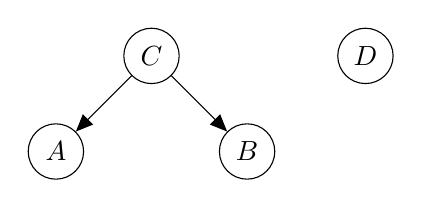
\begin{tikzpicture}
      \node[latent] (C) {$C$};
      \node[latent, below left = of C] (A) {$A$};
      \node[latent, below right = of C] (B) {$B$};
      \node[latent, right = 2 of C] (D) {$D$};
      \edge {C} {A, B};
    \end{tikzpicture}
  \]
  $a \land b \land c \land d$ will be split into $(a \land c) \land (b \land c)
  \land d$.
\end{enumerate}

\subsection{Bayesian networks as Boolean algebras}

\begin{table}
  \caption{Examples of how Bayesian networks encode as Boolean algebras. Here,
    $A$ denotes $\mathcal{F}\{a\}$ and $AB$ denotes $\mathcal{F}\{a, b\}$.}
  \centering
  \begin{tabular}{cc}
    \toprule
    Bayesian network & Boolean algebra \\
    \midrule \\[-1.3em]
    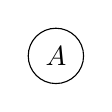
\begin{tikzpicture}[baseline={(A.base)}]
      \node[latent] (A) {$A$};
    \end{tikzpicture} & $A$ \\
    \midrule \\[-1.3em]
    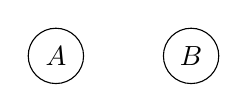
\begin{tikzpicture}[baseline={(A.base)}]
      \node[latent] (A) {$A$};
      \node[latent,right =of A] (B) {$B$};
    \end{tikzpicture} & $A + B$ \\
    \midrule \\[-1.3em]
    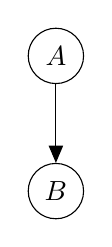
\begin{tikzpicture}[baseline={($(A.base)!.5!(B.base)$)}]
      \node[latent] (A) {$A$};
      \node[latent,below =of A] (B) {$B$};
      \edge {A} {B};
    \end{tikzpicture} & $AB$ \\
    \midrule \\[-1.3em]
    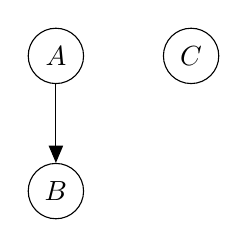
\begin{tikzpicture}[baseline={($(A.base)!.5!(B.base)$)}]
      \node[latent] (A) {$A$};
      \node[latent,below =of A] (B) {$B$};
      \node[latent,right =of A] (C) {$C$};
      \edge {A} {B};
    \end{tikzpicture} & $B +_A C$ \\
    \midrule \\[-1.3em]
    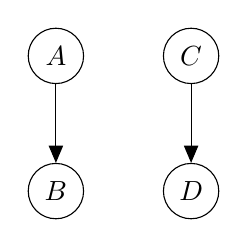
\begin{tikzpicture}[baseline={($(A.base)!.5!(B.base)$)}]
      \node[latent] (A) {$A$};
      \node[latent,below =of A] (B) {$B$};
      \node[latent,right =of A] (C) {$C$};
      \node[latent,below =of C] (D) {$D$};
      \edge {A} {B};
      \edge {C} {D};
    \end{tikzpicture} & $B +_{A+C} D$ \\
    \midrule \\[-1.3em]
    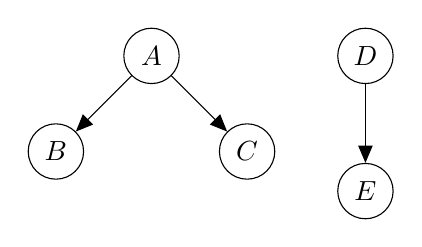
\begin{tikzpicture}[baseline={($(A.base)!.5!(B.base)$)}]
      \node[latent] (A) {$A$};
      \node[latent,below left =of A] (B) {$B$};
      \node[latent,below right=of A] (C) {$C$};
      \node[latent,right = 2 of A] (D) {$D$};
      \node[latent,below =of D] (E) {$E$};
      \edge {A} {B,C};
      \edge {D} {E};
    \end{tikzpicture} & $B +_{A+D} C +_{A+D} E$ \\
    \bottomrule
  \end{tabular}
\end{table}

To turn a Bayesian network into a Boolean algebra, run $f(\{ v \in V \mid
\mathrm{outdeg}(v) = 0 \})$, where $f$ works as follows on an arbitrary $A
\subseteq V$:
\begin{enumerate}
\item $S \gets \{ u \mid (u, v) \in E\text{, } v \in A \}$ (i.e., $S$ is the set
  of parents of the elements in $A$).
\item If $S = \emptyset$, return $\sum A$ (a coproduct).
\item Otherwise, return $\sum_{f(S)} A$ (a pushout).
\end{enumerate}

\bibliographystyle{plain}
\bibliography{paper}

\end{document}
